\documentclass[12pt,a4paper]{article}
\usepackage[utf8]{inputenc}
\usepackage[T1]{fontenc}
\usepackage{amsmath}
\usepackage{amsfonts}
\usepackage{amssymb}
\usepackage{multicol}
\usepackage{qrcode}
\usepackage{lmodern}
\usepackage{colortbl}%permet de griser les cases
\usepackage{tabularx, multirow}
%\usepackage{lscape}
\usepackage{xcolor}
%\usepackage{graphicx}
\usepackage{tikz,tkz-base}
\input{preambulemanu.sty}
\usepackage[left=2cm,right=2cm,top=2cm,bottom=2cm]{geometry}
\def\Oij{$\left(\text{O},~\vec{i},~\vec{j}\right)$}
\usepackage{fancyhdr}
\usepackage{MnSymbol,wasysym}

%Permet le code python sur lateX
\usepackage{minted}
\usemintedstyle{lovelace}

%Permet de mettre les coordonnées d'un vecteur
\newcommand*{\Coord}[3]{% 
  \ensuremath{\overrightarrow{#1}\, 
    \begin{pmatrix} 
      #2\\ 
      #3 
    \end{pmatrix}}}

\begin{document}
\textbf{1SPEmaths} \hfill \textbf{Produit scalaire} \hfill Lycée Jean Rostand\\
\trait 

\subsection*{Exercice n°1}

On considère le carré ABCD de centre O et de côté 8.

\begin{center}
  
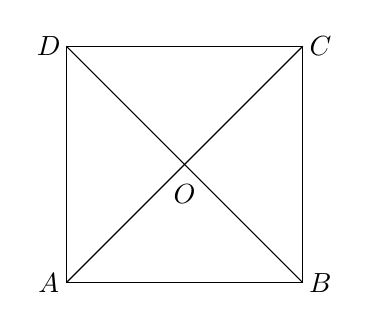
\begin{tikzpicture}[scale=0.75]
\draw  (0,0)-- (0,4);
\draw  (0,4)-- (4,4);
\draw  (4,4)-- (4,0);
\draw  (0,0)-- (4,4);
\draw  (0,4) -- (4,0);
\draw  (0,0) -- (4,0);

\draw  (-0.3,0) node {$A$};
\draw  (-0.3,4) node {$D$};
\draw  (4.3,4) node {$C$};
\draw (4.3,0) node {$B$};
\draw (2,1.5) node {$O$};
\end{tikzpicture}
\end{center}
Calculer les produits scalaire suivants:
\begin{enumerate}
\begin{minipage}[t]{0.4\linewidth}
\item $\vv{AB}.\vv{AO}$
\item $\vv{AB}.\vv{AD}$
\end{minipage}
\begin{minipage}[t]{0.4\linewidth}
\item $\vv{AB}.\vv{CD}$
\item $\vv{BO}.\vv{OD}$
\end{minipage}
\begin{minipage}[t]{0.4\linewidth}
\item $\vv{OB}.\vv{DO}$
\end{minipage}

\end{enumerate}

\subsection*{Exercice n°A}


On considère le carré ABCD de centre O et de côté 6.

\begin{center}
  
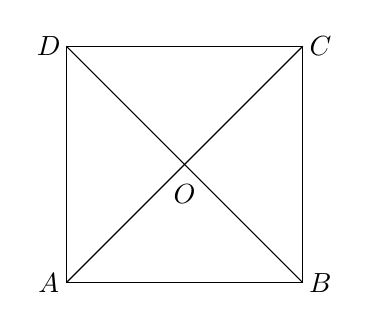
\begin{tikzpicture}[scale=0.75]
\draw  (0,0)-- (0,4);
\draw  (0,4)-- (4,4);
\draw  (4,4)-- (4,0);
\draw  (0,0)-- (4,4);
\draw  (0,4) -- (4,0);
\draw  (0,0) -- (4,0);

\draw  (-0.3,0) node {$A$};
\draw  (-0.3,4) node {$D$};
\draw  (4.3,4) node {$C$};
\draw (4.3,0) node {$B$};
\draw (2,1.5) node {$O$};
\end{tikzpicture}
\end{center}
Calculer les produits scalaire suivants:
\begin{enumerate}
\begin{minipage}[t]{0.4\linewidth}
\item $\vv{AD}.\vv{AO}$
\item $\vv{OB}.\vv{OD}$
\end{minipage}
\begin{minipage}[t]{0.4\linewidth}
\item $\vv{BO}.\vv{BC}$
\item $\vv{AO}.\vv{OC}$
\end{minipage}
\begin{minipage}[t]{0.4\linewidth}
\item $\vv{AB}.\vv{OD}$
\end{minipage}

\end{enumerate}


\subsection*{Exercice n°2}

ABCD est un rectangle (avec $AB=4$ et $AD=3$ ) de centre $F$ et $E$ est le symétrique de $F$ par rapport à (BC) .

\begin{center}
    
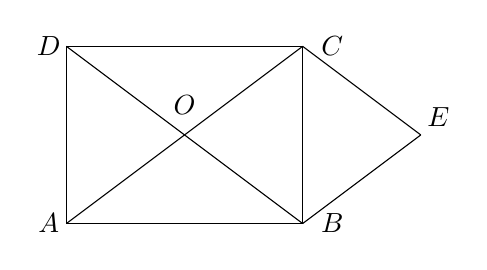
\begin{tikzpicture}[scale=0.75]
\draw  (0,0)-- (0,3);
\draw  (0,3)-- (4,3);
\draw  (4,3)-- (4,0);
\draw  (0,0)-- (4,3);
\draw (0,3)--(4,0);
\draw (0,0) -- (4,0);
\draw  (4,3) -- (6,1.5);
\draw  (4,0) -- (6,1.5);

\draw  (-0.3,0) node {$A$};
\draw  (-0.3,3) node {$D$};
\draw  (4.5,3) node {$C$};
\draw (4.5,0) node {$B$};
\draw (2,2) node {$O$};
\draw (6.3,1.8) node {$E$};
\end{tikzpicture}
\end{center}



Calculer les produits scalaires suivants:


\begin{enumerate}
\begin{minipage}[t]{0.4\linewidth}
\item $\vv{CF}.\vv{CD}$
\item $\vv{BA}.\vv{BE}$
\end{minipage}
\begin{minipage}[t]{0.4\linewidth}
\item $\vv{AF}.\vv{AB}$
\item $\vv{AB}.\vv{BE}$
\end{minipage}
\begin{minipage}[t]{0.4\linewidth}
\item $\vv{BF}.\vv{DC}$
\item $\vv{AF}.\vv{BE}$
\end{minipage}

\end{enumerate}

\subsection*{Exercice n°3}

Dans chacun des cas suivants, calculer le produit scalaire de $\vv{u}$ par $\vv{v}$:

\begin{enumerate}
\begin{minipage}[t]{0.5\linewidth}
\item $\norme{\vv{u}}=2$, $\norme{\vv{v}}=3$ et $(\vv{u};\vv{v})=60^\circ $
\item $\norme{\vv{u}}=1$, $\norme{\vv{v}}=4$ et $(\vv{u};\vv{v})=\dfrac{\pi}{3} $
\end{minipage}
\begin{minipage}[t]{0.5\linewidth}
\item $\norme{\vv{u}}=8$, $\norme{\vv{v}}=\sqrt{2}$ et $(\vv{u};\vv{v})=\dfrac{3\pi}{4} $
\item $\norme{\vv{u}}=5$, $\norme{\vv{v}}=\sqrt{3}$ et $(\vv{u};\vv{v})=135^\circ $
\end{minipage}
\end{enumerate}


\subsection*{Exercice n°4}

Déterminer une valeur en radian de l'angle de vecteur $(\vv{u};\vv{v})$ dans chacun des cas suivants:

\begin{enumerate}
    \item $\norme{\vv{u}}=6$, $\norme{\vv{v}}=2$ et $(\vv{u}.\vv{v})=-6 $
    \item $\norme{\vv{u}}=2$, $\norme{\vv{v}}=\sqrt{3}$ et $(\vv{u}.\vv{v})=\sqrt{6} $
\end{enumerate}

\subsection*{Exercice n°5}

On considère le carré ABCD de côté $5$.\\ Calculer le produit scalaire $\vv{AB}.\vv{AC}$\\
On passera par la définition avec le cosinus et on pourra réaliser un dessin à main levée pour visualiser la situation.

\subsection*{Exercice n°6}

Dans un repère \Oij{}:

\begin{enumerate}
    \item On pose $\Coord{u}{2}{-3}$ et $\Coord{v}{4}{\frac{5}{3}}$. Calculer $\vv{u}.\vv{v}$ 
    \item On pose $\Coord{w}{5}{-3}$ et $\Coord{t}{2}{y}$. Déterminer $y$ sachant que $\vv{w}.\vv{t}=1$ 
\end{enumerate}

\subsection*{Exercice n°7}

Soient les vecteurs $\Coord{u}{-2}{3}$ et 
$\Coord{v}{-1}{-5}$. Calculer:

\begin{enumerate}
\begin{minipage}[t]{0.4\linewidth}
\item $\vv{u}.\vv{v}$

\end{minipage}
\begin{minipage}[t]{0.4\linewidth}
\item $(4\vv{u}).\vv{v}$

\end{minipage}
\begin{minipage}[t]{0.4\linewidth}
\item $(\vv{u}-\vv{v})(\vv{u}+\vv{v})$
\end{minipage}
\end{enumerate}

\subsection*{Exercice n°8}

Soient les vecteurs $\Coord{u}{2}{1}$ et 
$\Coord{v}{-3}{-1}$ et $\Coord{w}{1}{4}$. Calculer:

\begin{enumerate}
\begin{minipage}[t]{0.3\linewidth}
\item $\vv{u}.\vv{v}$

\end{minipage}
\begin{minipage}[t]{0.3\linewidth}
\item $\vv{w}.\vv{v}$

\end{minipage}
\begin{minipage}[t]{0.3\linewidth}
\item $\vv{u}.(\vv{v}+\vv{w})$
\end{minipage}

\begin{minipage}[t]{0.3\linewidth}
\item $(-2\vv{u}).\vv{v}+3(\vv{v}.\vv{w})$
\end{minipage}

\end{enumerate}


\subsection*{Exercice n°9}

On considère les points $A(-2;3)$, $B(-1;-2)$ , $C(0,4)$ et $D(2;5)$. Calculer:

\begin{enumerate}
\begin{minipage}[t]{0.2\linewidth}
\item $\vv{AB}.\vv{BC}$

\end{minipage}
\begin{minipage}[t]{0.2\linewidth}
\item $\vv{CB}.\vv{BD}$

\end{minipage}
\begin{minipage}[t]{0.2\linewidth}
\item $\vv{AB}.\vv{CD}$
\end{minipage}

\begin{minipage}[t]{0.2\linewidth}
\item $\vv{BA}.\vv{AD}$
\end{minipage}

\end{enumerate}

\subsection*{Exercice n°B}

Dans un repère orthonormé du plan, on considère les point A,B et C dont les coordonnées respectives sont $(-2;-2)$, $(3;1)$ et $(-1;2)$.
\begin{enumerate}
    \item 
    \begin{enumerate}
        \item Calculer les coordonnées $\vv{AB}$ et $\vv{AC}$
        \item En déduire la valeur du produit scalaire $\vv{AB}.\vv{AC}$
    \end{enumerate}
    \item
    \begin{enumerate}
        \item Calculer les distances $AB$ et $AC$
        \item En déduire une valeur de l'angle $\widehat{BAC}$ en radian
    \end{enumerate}

\end{enumerate}

\subsection*{Exercice n°10} 

On se situe dans un repère orthonormé du plan

\begin{enumerate}
    \item Montrer que les vecteurs $\Coord{u}{-3}{4}$ et $\Coord{v}{-8}{-6}$ sont orthogonaux.
    \item On donne les points $A(-3;-2)$ et $B(1;3)$ et le vecteur $\Coord{u}{-5}{4}$. \\
    Montrer que $\vv{AB}$ et $\vv{u}$ sont orthogonaux.
\end{enumerate}

\subsection*{Exercice n°C} 

Dans un repère orthonormé du plan, on donne $A(5;3)$, $B(8;-5)$, $C(-1;0)$ et $D(3;1,5)$.\\
Montrer que $(AB)$ et $(CD)$ sont perpendiculaires.


\subsection*{Exercice n°11} 
Dans les cas suivants:

\begin{enumerate}
    \item Dire si les vecteurs $\vv{u}$ et $\vv{v}$ sont orthogonaux:
    \begin{enumerate}
        \item $\Coord{u}{-1}{3}$ et $\Coord{v}{3}{-1}$
        \item $\Coord{u}{2}{4}$ et $\Coord{v}{-6}{3}$
    \end{enumerate}
    \item Dire si les droites $(AB)$ et $(CD)$ sont perpendiculaires:
    \begin{enumerate}
        \item $A(2;-3)$ , $B(-1;-1)$, $C(5;-3)$ et $D(2;1)$
        \item $A(-1;-2)$ , $B(-2;-4)$, $C(7;-1)$ et $D(3;1)$
    \end{enumerate}
    \item Déterminer la ou les valeurs de $a$ pour que $\vv{u}$ et $\vv{v}$ soient orthogonaux:
    \begin{enumerate}
        \item $\Coord{u}{-5}{4}$ et $\Coord{v}{1}{a}$
        \item $\Coord{u}{2}{a+1}$ et $\Coord{v}{a+5}{3}$
        \item $\Coord{u}{a}{-3+a}$ et $\Coord{v}{2}{a}$
    \end{enumerate}
\end{enumerate}

\newpage
\subsection*{Exercice n°12} 

Donner un vecteur directeur pour chacune des droites suivantes et en déduire qu'elles sont perpendiculaires.

\begin{enumerate}
    \item $\mathscr{D}_{1}:2x-3y+4=0$ et $\mathscr{D}_2:3x+2y-1=0$
    \item $\mathscr{D}_{1}:x-y+3=0$ et $\mathscr{D}_2:2x+2y-1=0$
    \item $\mathscr{D}_{1}:y=3x+1$ et $\mathscr{D}_2:-x+3y-1=0$
\end{enumerate}

\begin{raps}

Une droite $\mathscr{D}$ d'équation cartésienne $ax+by+c=0$ a pour vecteur directeur $\Coord{u}{-b}{a}$.\\

Une droite d'équation réduite $y=ax+b$ a pour vecteur directeur $\Coord{v}{1}{a}$.
\end{raps}


\subsection*{Exercice n°13} 

Déterminer une équation de la médiatrice du segment $[AB]$ avec $A(3,-5)$ et $B(1;4)$ dans un repère orthonormé \Oij{}
\textit{On pourra faire un dessin à main levée pour visualiser la situation donnée}

\subsection*{Exercice n°14} 

On considère deux carrés $ABCD$ et $BEFG$ disposés comme sur la figure ci-dessous tel que $AB=1$ et $BE=a$


\begin{center}
  
\begin{tikzpicture}[scale=1]
\draw  (0,0)-- (0,1);
\draw  (0,1)-- (1,1);
\draw  (1,1)-- (1,0);
\draw  (0,0) -- (1,0);
\draw  (1,0)-- (1,2);
\draw  (1,2)--(3,2);
\draw (3,2)-- (3,0);
\draw (3,0)--(1,0);
\draw[dash pattern=on 1mm off 1mm] (-1,-2)--(2,4);
\draw[dash pattern=on 1mm off 1mm] (5,-1)--(-1,2);

\draw  (0,0) node[left] {$A$};
\draw  (0,1) node [left]{$D$};
\draw  (1,1) node[above,right] {$C$};
\draw  (1,0) node[below] {$B$};
\draw  (3,0) node[right] {$E$};
\draw  (1,2) node[left] {$G$};
\draw  (3,2) node[right] {$F$};
\end{tikzpicture}
\end{center}

\textbf{Partie A: avec coordonnées}
\begin{enumerate}
    \item Dans le repère $(A;B;D)$ , donner les coordonnées de tous les points de la figure.
    \item  Démontrer que les droites $(AG)$ et $(CE)$ sont perpendiculaires.
\end{enumerate}

\textbf{Partie B: sans coordonnées}

\begin{enumerate}
    \item Développer le produit scalaire $(\vv{AB}+\vv{BG}).(\vv{CB}+\vv{BE})$
    \item En déduire que $\vv{AG}.\vv{CE}=0$ et conclure.
\end{enumerate}

\newpage
\subsection*{Exercice n°D} 

Soit $a$ un nombre réel positif. On considère le rectangle $ABCD$ tel que $AB=a$ et $AD=\dfrac{\sqrt{2}}{2}a$.
On note $I$ milieu de $[CD]$.


\begin{center}
  
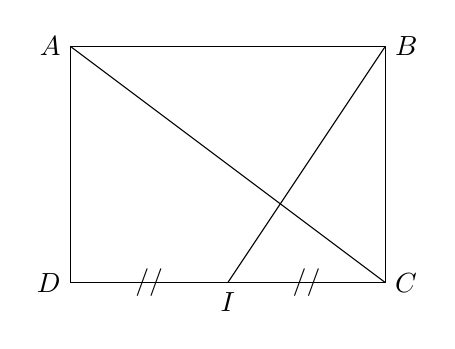
\begin{tikzpicture}[scale=1]
\draw  (0,3)-- (4,3);
\draw  (4,3)-- (4,0);
\draw  (4,0)-- (0,0);
\draw  (0,0) -- (0,3);
\draw  (0,3)-- (4,0);
\draw  (2,0)--(4,3);



\draw  (0,0) node[left] {$D$};
\draw  (0,3) node [left]{$A$};
\draw  (4,3) node[right] {$B$};
\draw  (4,0) node[right] {$C$};
\draw  (2,0) node[below] {$I$};
\draw (1,0) node {$//$};
\draw (3,0) node {$//$};
\end{tikzpicture}
\end{center}

En se servant uniquement des propriétés algébriques, démontrer que les droites $(AC)$ et $(BI)$ sont perpendiculaires.

\subsection*{Exercice n°E} 

On considère la figure ci-dessous.

\begin{enumerate}
    \item Calculer la longueur $BC$
    \item Calculer la longueur $CD$
    \item En déduire la mesure de l'angle $\widehat{BDC}$ en degrés arrondie au dixième 
\end{enumerate}


\begin{center}
  
\begin{tikzpicture}[scale=0.75]
\draw  (0,0)-- (4.48,4.32);
\draw  (4.48,4.32)-- (11,0);
\draw  (4.48,4.32)-- (7,0);
\draw  (0,0) -- (7,0);
\draw  (7,0)-- (11,0);




\draw  (0,0) node[left] {$D$};
\draw  (7,0) node [below]{$A$};
\draw  (11,0) node[right] {$B$};
\draw  (4.48,4.32) node[above] {$C$};
\draw  (7,0) ++(0:1) arc(0:120:1);
\draw (7.4,0.35) node {$120^\circ$};
\draw (3.5,0) node[below]{$7$};
\draw (6,2) node[right]{$5$};
\draw (9,0) node[below]{$4$};
\end{tikzpicture}
\end{center}


\subsection*{Exercice n°15} 

On considère les points A, B et C tels que $AB=3$, $AC=4$ et $\widehat{BAC}=120^\circ$.\\
Déterminer la longueur $BC$.\\
On pourra réaliser une figure à main levée pour visualiser la situation.


\subsection*{Exercice n°16} 

On considère les points M,N et P tels que $MN=5$, $NP=7$ et $\widehat{MNP}=61^\circ$.\\
Déterminer la longueur MP.

\subsection*{Exercice n°17} 

Soit un triangle $EFG$ tel que $EF=7$, $FG=6$ et $EG=11$.\\
Déterminer la valeur en degrés et arrondie au dixième de l'angle $\widehat{EFG}$

\subsection*{Exercice n°18} 

Soit un triangle $EFG$ tel que $EF=5$, $FG=8$ et $\widehat{EFG}=60^\circ$.\\

\begin{enumerate}
    \item Déterminer la valeur exaxte de $EG$, puis une valeur approchée  arrondie au dixième.
    \item Déterminer une valeur approchée de $\widehat{FGE}$ arrondie à l'unité.
\end{enumerate}

\subsection*{Exercice n°19} 

On donne les points A et B tels que $AB=12$ et $I$ le milieu du segment $[AB]$.\\
Déterminer l'ensemble des points $M$ du plan vérifiant $\vv{MA}.\vv{MB}=4$

\subsection*{Exercice n°20} 

On donne les points C et D tels que $CD=10$ et $H$ le milieu du segment $[CD]$.\\
Déterminer l'ensemble des points $M$ du plan vérifiant $\vv{MC}.\vv{MD}=-9$

\subsection*{Exercice n°21} 

On considère les points $A(-2;-3)$ et $B(-1;4)$.\\

\begin{enumerate}
    \item Calculer la longueur $AB$
    \item Déterminer les coordonnées du milieu du segment $[AB]$
    \item Déterminer l'ensemble des points $M$ du plan vérifiant $\vv{MA}.\vv{MB}=0$
\end{enumerate}

\subsection*{Exercice n°22} 

On considère un triangle $ABC$ et $A'$ est le milieu du segment $[BC]$.\\
Déterminer l'ensemble des points $M$ du plan vérifiant $\vv{MA}.(\vv{MB}+\vv{MC})=0$

\subsection*{Exercice n°23} 

On considère deux points $C$ et $V$ tels que $CV=8$.\\
Déterminer l'ensemble des points $M$ tels que $\vv{CM}.\vv{VM}=-4$




\end{document}

